This section demonstrates the practical results of the proposed approach application. We introduce an easy-to-use implementation, specify some experimental details and describe currently available models. We compare our results with several popular tools and show the competitive power of our models.

\subsection{Tool}
The proposed approach was implemented as a Python console tool Genegram. Code, installation instructions, and documentation are available by link \linebreak \url{https://github.com/JetBrains-Research/Genegram}. This tool accepts a file with RNA sequences in fasta format and returns the connectivity tables (ct) for the corresponding secondary structures. We use an effective Python implementation of the parsing algorithm~\cite{Azimov:2018:CPQ:3210259.3210264} that shows high performance due to the GPGPU utilization and Keras~\cite{chollet2015keras} library with Tensorflow-GPU~\cite{tensorflow2015-whitepaper} framework for running the predictive model. Genegram tool allows to select different models and process sequences of lengths 1-200 containing only four canonical nucleotides.

\subsection{Setup}
The approach itself is quite flexible and Genegram tool provides a convenient environment for different experiments allowing to change both grammar and network. However, in the present work, we freeze grammar $G_0$ from figure~\ref{gram} and parallel ResNet architecture from figure~\ref{nn} with $k := 10$, $n := 4$. We consider only small RNAs (lengths from 1 to 200) due to the insufficient amount of longer sequences in biological databases and GPU storage limitations. Each sequence of $l$ nucleotides results in the image of size $l \times l$, therefore, images are grouped into batches by image size and cyclically duplicated until all batches have the same length. We use two data augmentation techniques on the training dataset: firstly, we mirror each image along the main diagonal (so that mirrored image represents the same sequence turned backwards), and secondly, we copy both regular and mirrored images twice. On this data, we run 10-fold cross-validation in order to choose the best train and validation split for each model.

The quality of the results is estimated by classical machine learning metrics calculated on the pixel-by-pixel difference between predicted and reference images. Further, we consider $TP$ (true positives, i.e. true white pixels), $FP$ (false positives, i.e. false white pixels), and $FN$ (false negatives, i.e. false black pixels) as numbers of right and wrong decisions among all contacts and calculate three following metrics for each image of some dataset. 

\begin{itemize} 
    \item $Precision = \displaystyle \frac{TP}{TP + FP}$ (proportion of correct contacts among all detected).
    \item $Recall = \displaystyle \frac{TP}{TP + FN}$ (proportion of detected contacts among all expected).
    \item $F1 = \displaystyle 2 * \frac{Precision * Recall}{Precision + Recall}$ (harmonic mean --- aggregation metrics).
\end{itemize}

The loss function is based on the idea of maximizing $F1$ score and that is to be achieved by minimizing the dataset mean $1 - F1$ through gradient descent. However, $F1$ is not differentiable as a function, so, we replace the sums of discrete integer values with a continuous sum of probabilities. Also, we charge our loss with two penalty coefficients responsible for huge dispersion between $Precision$ and $Recall$ for each image ($k1$) and the whole dataset ($k2$). Figure~\ref{loss} demonstrates the Python code for the currently used  $F1\_loss$ function that accepts two arguments: predicted image $y\_p$ and true image $y\_t$.

\begin{figure}[h]
\centering
\begin{lstlisting}[language=Python]
from keras import backend as K

def f1_loss(y_t, y_p):
    #normalize pixels values to [0, 1]
    y_t, y_p = K.minimum(y_t / 255, 1), K.minimum(y_p / 255, 1)
    #calculate differentiable versions of tw, fw and fb
    tw = K.sum(K.cast(y_t * y_p, 'float32'), axis=[1, 2, 3])
    fw = K.sum(K.cast((1 - y_t) * y_p, 'float32'), axis=[1, 2, 3])
    fb = K.sum(K.cast(y_t * (1 - y_p), 'float32'), axis=[1, 2, 3])
    #calculate precision and recall secure from zero division error
    prec = tw / (tw + fw + K.epsilon())
    rec = tw / (tw + fb + K.epsilon())
    #penalties for huge difference between precision and recall 
    #calculated for each image and whole dataset respectively
    k1 = 1 -  K.abs(prec- rec)
    k2 = 1 -  K.abs(K.mean(prec) - K.mean(rec))
    #calculate upgraded f1 score and return its mean value
    f1 = k1 * k2 * 2 * prec * rec / (prec + rec + K.epsilon()) 
    return 1 - K.mean(f1)
\end{lstlisting}
\caption{$F1\_loss$ function}
\label{loss}
\end{figure} 

For hyperparameters, we use Dropout after each residual unit to deal with overfitting, L2-regularization that also prevents overfitting and allows to search for complex data patterns, and Adagrad optimizer that automatically sets the learning rate and is known to be a powerful solution for sparse data processing.

For a comparative analysis of the results we selected six tools based on various concepts and algorithms. All of them demonstrate adequate speed and high accuracy, can handle pseudoknots and are easy to launch and use.

\begin{itemize}
    \item SPOT-RNA~\cite{singh2019rna} --- deep neural networks + transfer learning.
    \item Ipknot~\cite{sato2011ipknot} --- MEA + integer programming.
    \item Knotty~\cite{jabbari2018knotty} --- MFE + sparse dynamic programming.
    \item RNAstructure~\cite{bellaousov2013rnastructure} --- MFE + dynamic programming. 
    \item PknotsRG~\cite{reeder2007pknotsrg} --- MFE + Turner energy rules.
    \item HotKnots~\cite{ren2005hotknots} --- MFE + heuristic algorithm.
\end{itemize}

\subsection{Models}
In these conditions, we trained three identical networks on three different datasets and compared them with each other and with other tools by several criteria. All three models are available to use in the Genegram tool and the default model here is Genegram-main. Let us describe the specifics of each dataset, present the results of the best 10-fold cross-validation splits, and draw some conclusions.

\subsubsection{Genegram-main}
The first model was trained on data obtained from RNA STRAND database~\cite{andronescu2008rna} that is quite popular in different RNA analysis research due to its quality and usability. This database is an assembly of carefully curated and validated RNA sequences with secondary structures collected from different sources, and it contains only trustful structures obtained by reliable methods (laboratory or comparative). This database is supposed to provide the most representative sample of RNA secondary structures along with a guaranteed high quality of data which makes Genegram-main model trained on RNA STRAND the most general one for now, therefore, we set it as a default choice for our tool.

We selected 1091 sequences with lengths up to 200 and removed samples with gaps or inaccuracies in primary and secondary structures. The distribution of sequences lengths in the prepared dataset is demonstrated in figure~\ref{main_distr}. Neural network output images are grayscale and may contain multiple contacts, therefore, we applied binarization by threshold 0.6 with multiplets removal as postprocessing for this model and calculated the following metrics afterwards. Figure~\ref{main_f1} shows the estimation of Genegram-main and other six tools on validation set of size 109 by metrics $F1$. The shape of colored plots shows the density of $F1$ values, the red line represents its median result and the blue line corresponds to the mean one. It can be seen that Genegram-main has median $F1$ equal to 81 (as well as Knotty which is the second result after SPOT-RNA), and mean $F1$ equal to 70 that significantly exceeds the results of all competing tools except SPOT-RNA. The estimation on the same set by mean $Precision$ and $Recall$ metrics is presented in figure~\ref{main_pr}. Note that the binarization threshold allows us to slightly manipulate the balance between these two metrics and we choose it so that $F1$ mean value is the highest, even though it leads to a small excess of $Precision$ over $Recall$.

\begin{figure}[h]
\centering
    \subfloat[$F1$ distribution, mean, \\ and median on valid set]
        {\label{main_f1}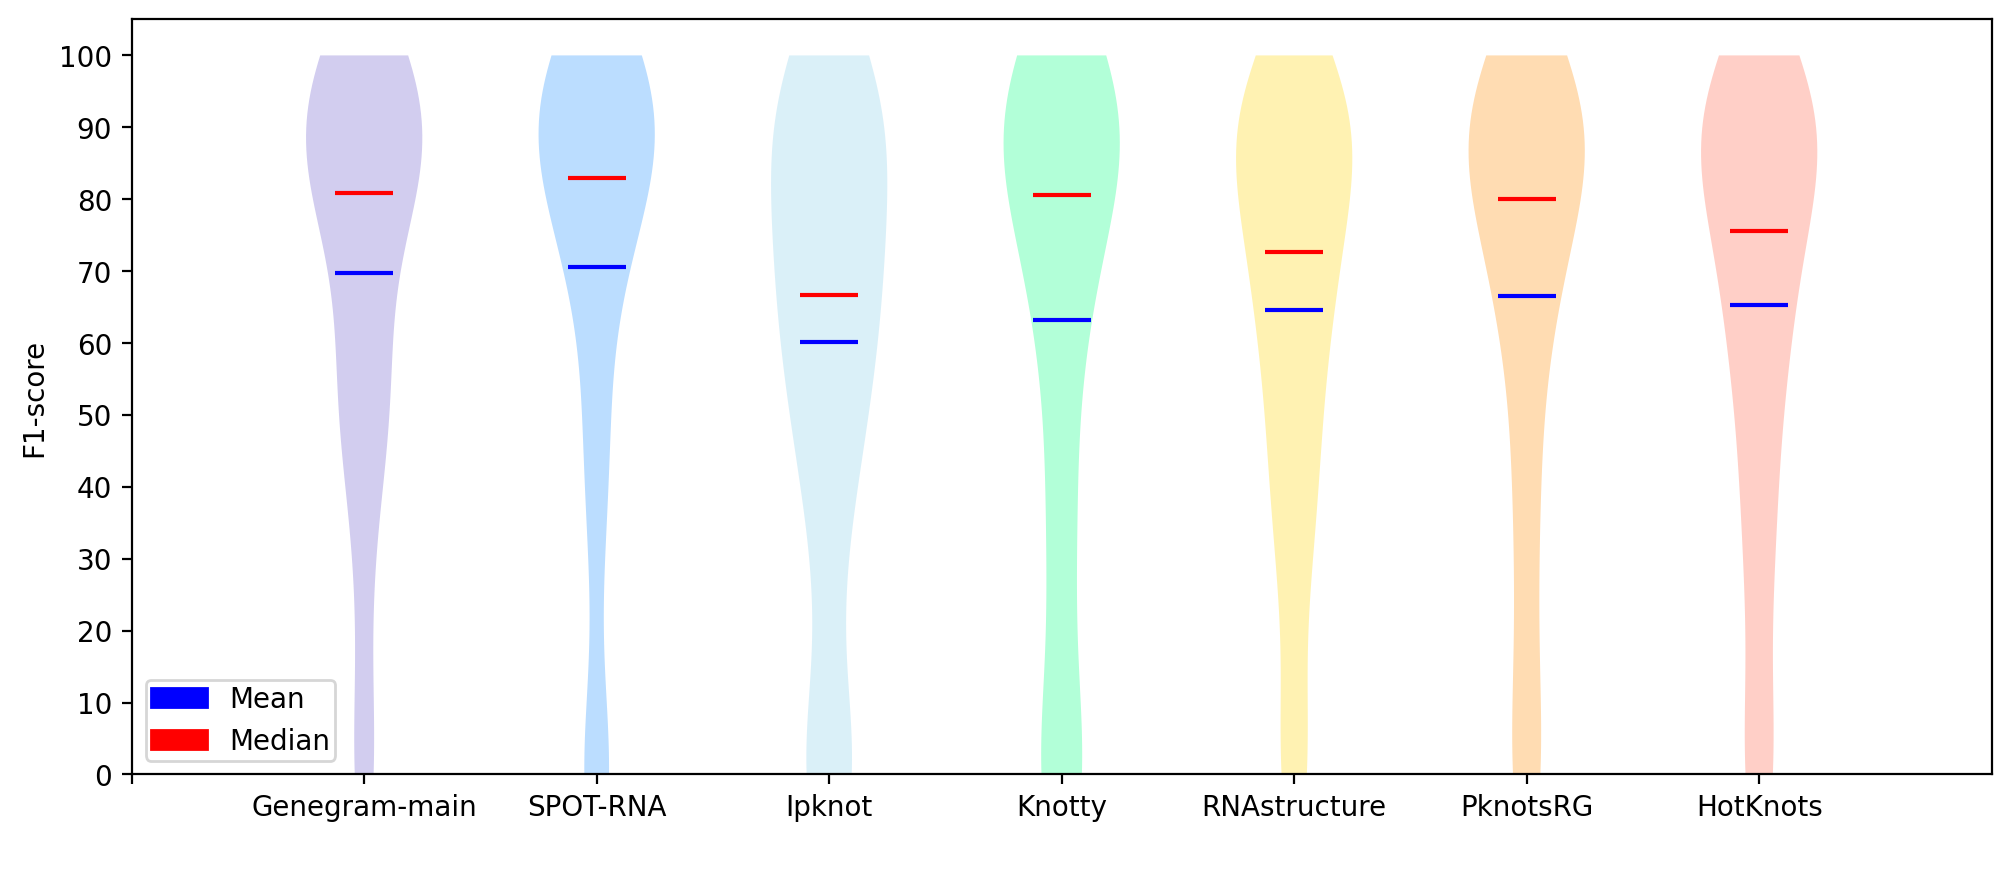
\includegraphics[width=.69\linewidth]{pics/plot_main_f1.png}}\hfill
    \subfloat[$Precision$ and $Recall$ mean on valid set]
        {\label{main_pr}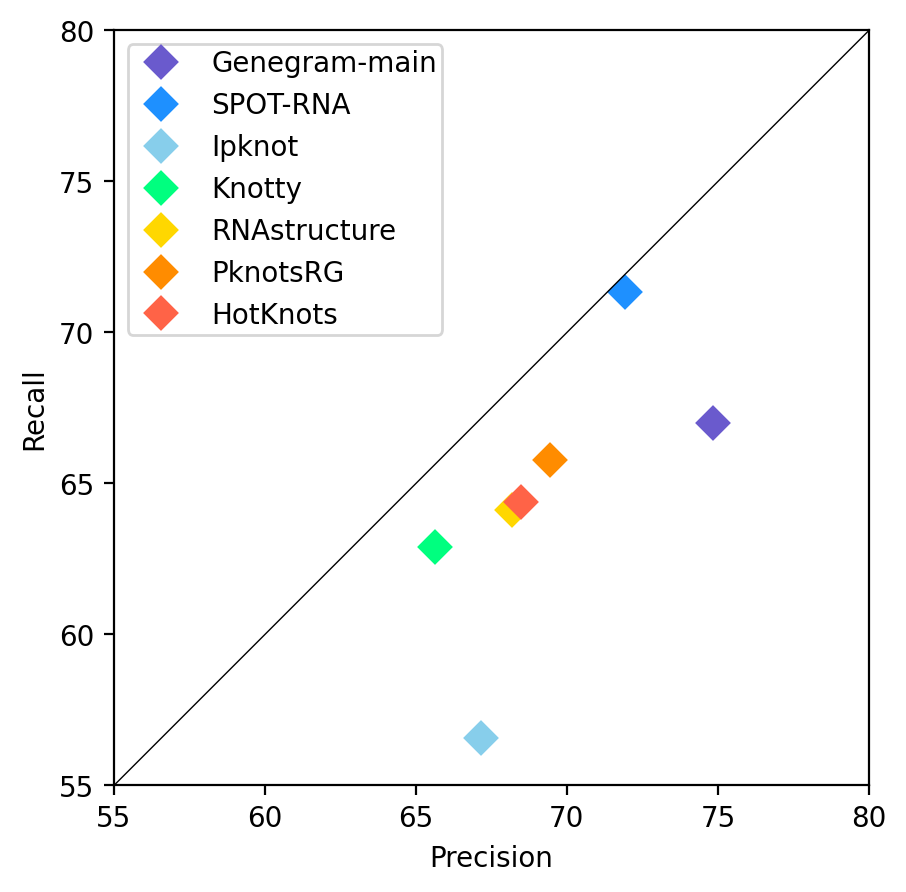
\includegraphics[width=.31\linewidth]{pics/plot_main_pr.png}}\par 
    \subfloat[Sequences lengths distribution on total set]
        {\label{main_distr}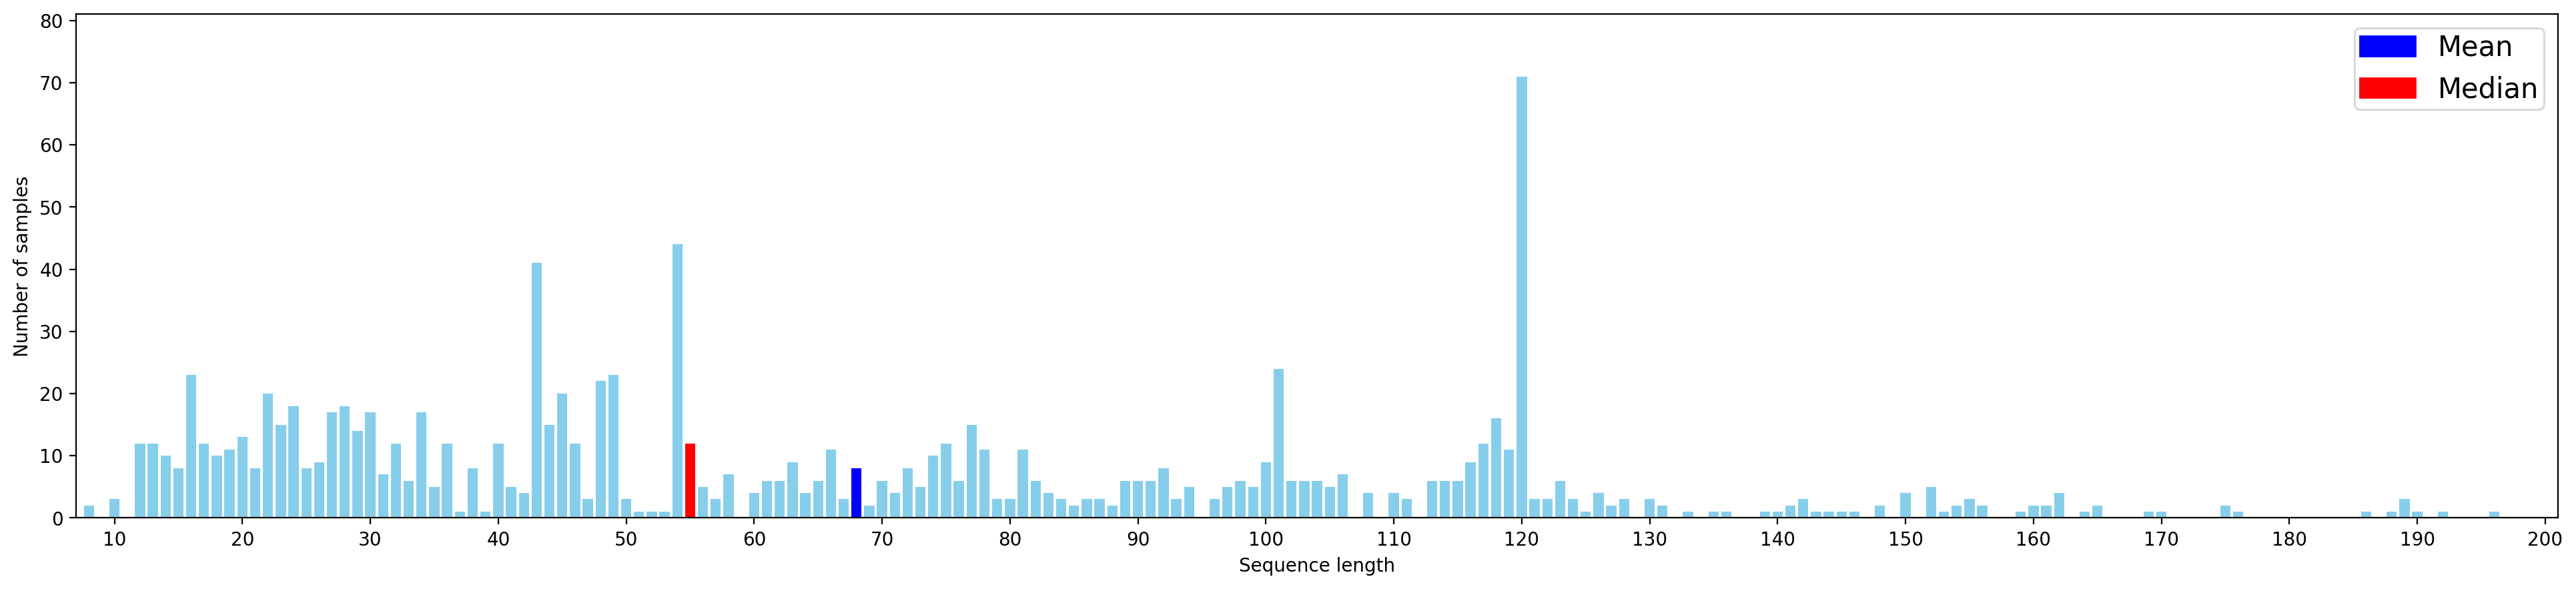
\includegraphics[width=\linewidth]{pics/plot_main_distr.png}}
\caption{Analysis of Genegram-main model compared with other tools }
\label{plots_main}
\end{figure}

All models were also estimated by several more specific functional criteria, such as pseudoknots prediction accuracy and sensitivity to different types of base pairs, so, table~\ref{table_main} demonstrates the results of these experiments. Considered validation set contained 11 pseudoknots and we calculated the number of correctly predicted contacts for each pseudoknot in each model output. The second column of table~\ref{table_main} shows the number of perfectly detected pseudoknots and the third column --- the number of ones that had up to 25\% extra or missing contacts. Clearly, pseudoknotted structures prediction is a non-trivial task for almost all models including Genegram-main. The other three columns of table~\ref{table_main} demonstrate how these tools handle different types of base pairs. Watson-Crick pairs are the most common and stable ones and it can be seen that all models have high enough canonical pairs prediction accuracy. Besides, it is known that wobble base pairs also have a biological role and regularly appear in real-world data, especially GU pair that has stability close to the Watson-Crick bonds. Our model slightly loses to other tools in GU pairs prediction, however, the great advantage of our approach is that it does not limit any types of pairs to be presented in neural network output (as well as SPOT-RNA that also uses neural networks), so, Genegram-main and SPOT-RNA are able to handle seven more wobble base pairs (AA, AC, AG, CC, CU, GG, UU), unlike other considered tools.

\begin{table}[h!]
\centering
\caption{Genegram-main and other models quality criteria measured on valid set}
\ra{1.4}
\begin{tabular}{@{}lccccccc@{}}\toprule
& \multicolumn{2}{c}{Pseudoknots} & \phantom{abc}& \multicolumn{3}{c}{Base pairs} \\
& No errors & 25\% errors  && Watson-Crick & GU & Others \\ \cmidrule{2-3} \cmidrule{5-7} 
Genegram-main  & 0 & 3 && 1067 & 68 & 53 \\
SPOT-RNA & 1 & 4 && 1190 & 134 & 39 \\
Ipknot & 0 & 1 && 939 & 92 & 0 \\
Knotty &1 & 3 && 1093 & 126 & 0 \\
RNAstructure & 1 & 1 && 1113 & 119 & 0 \\
PknotsRG & 1 & 5 && 1157 & 123 & 0 \\
HotKnots & 1 & 2 && 1113 & 112 & 0 \\
\bottomrule
Expected & 11 & 11 && 1650 & 185 & 135 \\
\bottomrule
\end{tabular}
\label{table_main}
\end{table}

\subsubsection{Genegram-pks}
Although the main model shows high results in general, it has poor pseudoknots prediction accuracy because RNA STRAND database contains only 86 sequences with pseudoknots and the neural network has not enough data to learn them, moreover, the amount of pseudoknots in the considered validation set is not enough to draw any conclusions. To improve this, we extended the previous dataset with sequences from Pseudobase~\cite{van2000pseudobase} database that is known to be a carefully built collection of pseudoknotted structures. Even though this database mostly contains not the whole sequences but only fragments with pseudoknots, we believe that the presence of such data in the training set may allow us to reach higher results in pseudoknots prediction.

We selected 1447 sequences having lengths up to 200 with no gaps or inaccuracies in primary and secondary structures and applied the same binarization by threshold 0.6 with multiplets removal as postprocessing. Note that both times we used 10-fold cross-validation on randomly shuffled data, so, Genegram-pks has separate from Genegram-main validation set, even though samples may intersect. Figure~\ref{pks_distr} shows the distribution of sequences lengths in total Genegram-pks dataset, figure~\ref{pks_f1} estimates all seven models on 145 validation sequences by $F1$ and figure~\ref{pks_pr} --- by $Precision$ and $Recall$ metrics. Genegram-pks is behind two tools by mean $F1$ value (70) and behind three tools by median (75) one, so, these results are quite competitive, however, Genegram-main was able to achieve the higher numbers.

\begin{figure}
\centering
    \subfloat[$F1$ distribution, mean, \\ and median on valid set]
        {\label{pks_f1}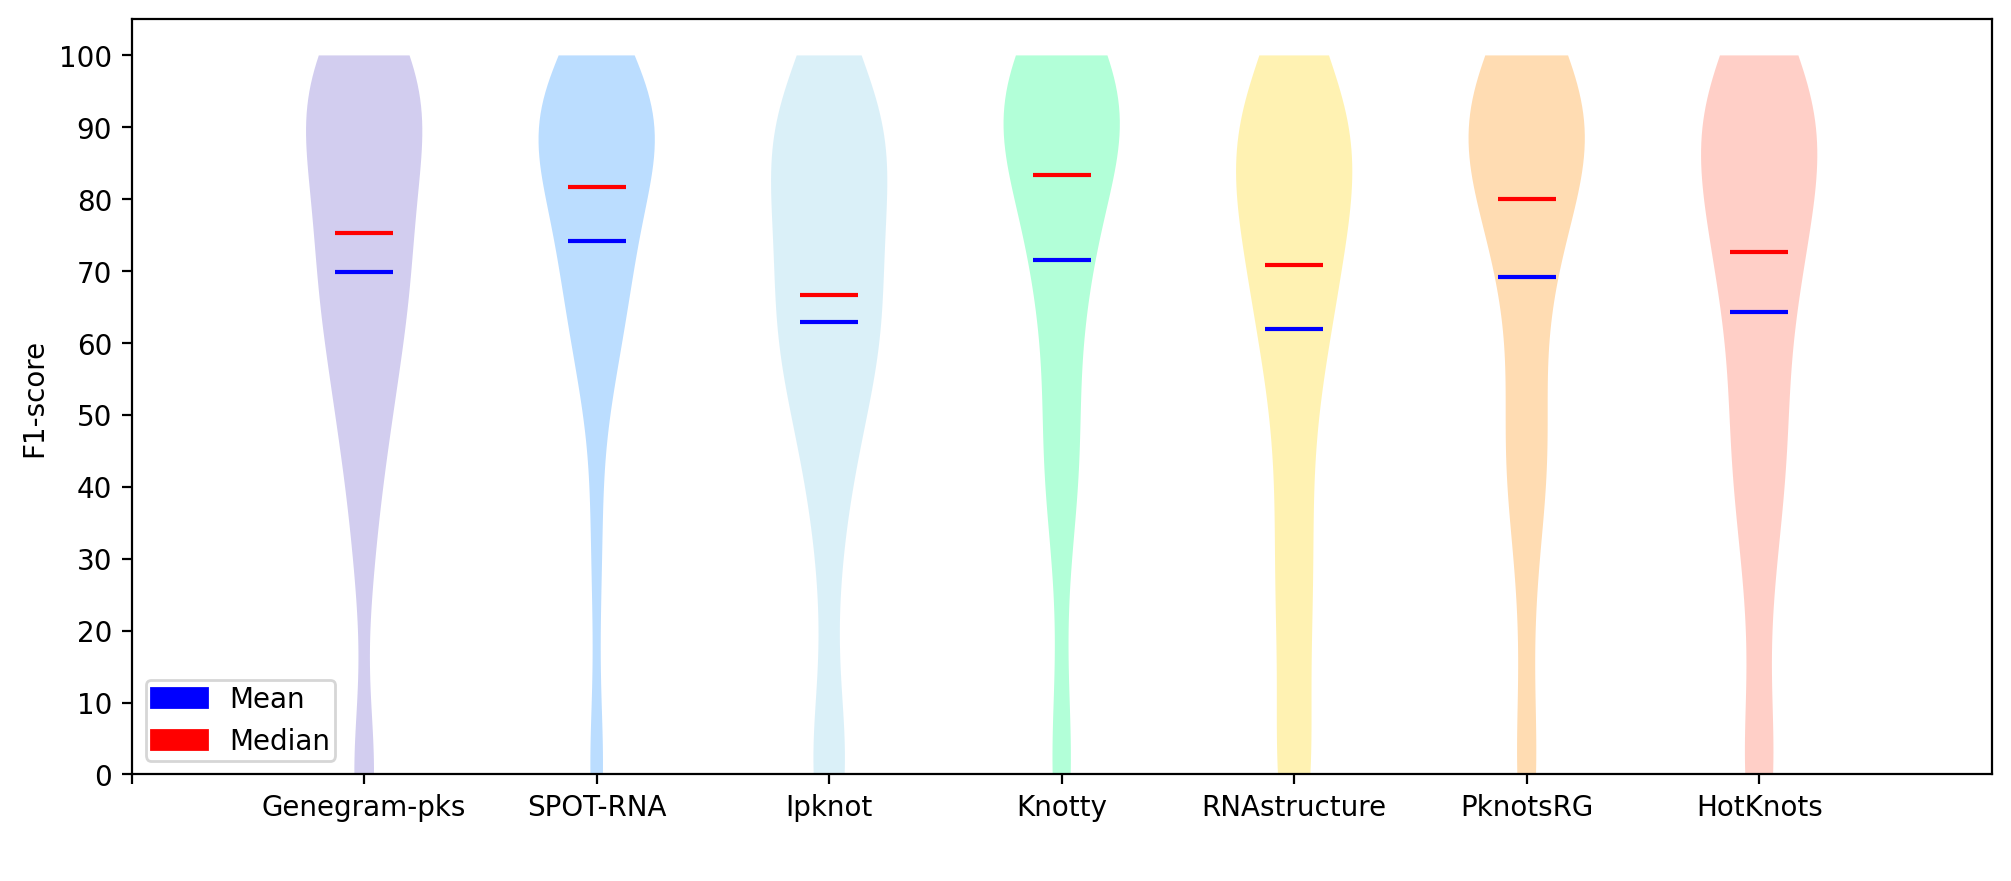
\includegraphics[width=.69\linewidth]{pics/plot_pks_f1.png}}\hfill
    \subfloat[$Precision$ and $Recall$ mean on valid set]
        {\label{pks_pr}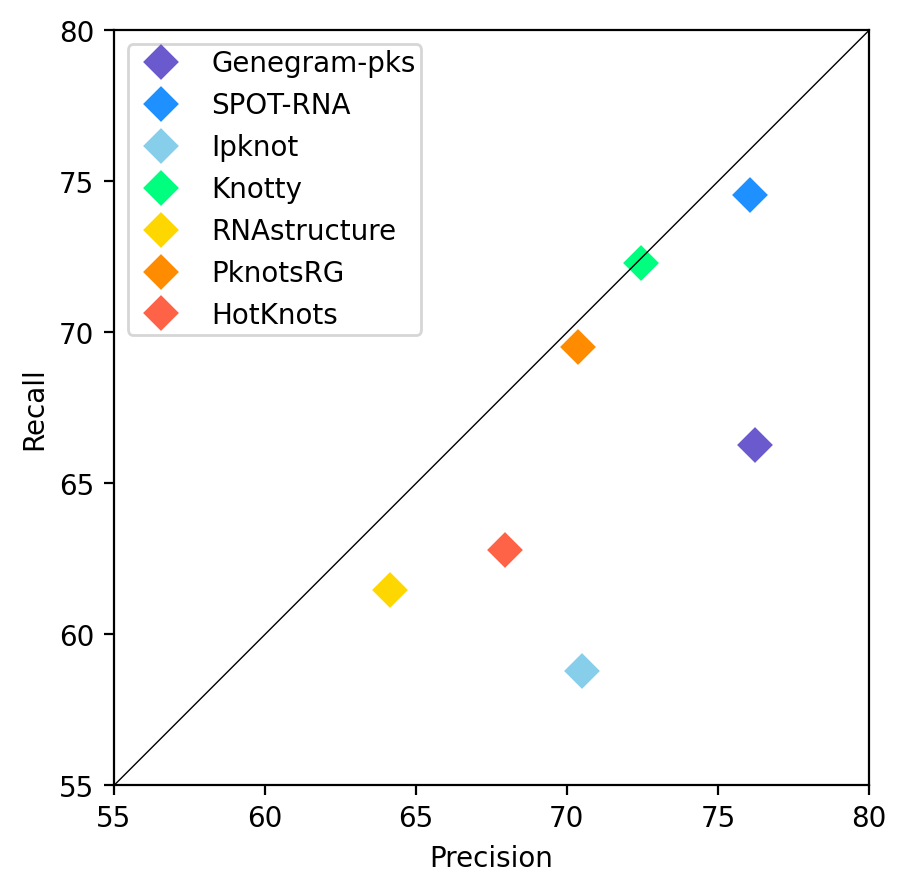
\includegraphics[width=.31\linewidth]{pics/plot_pks_pr.png}}\par 
    \subfloat[Sequences lengths distribution on total set]
        {\label{pks_distr}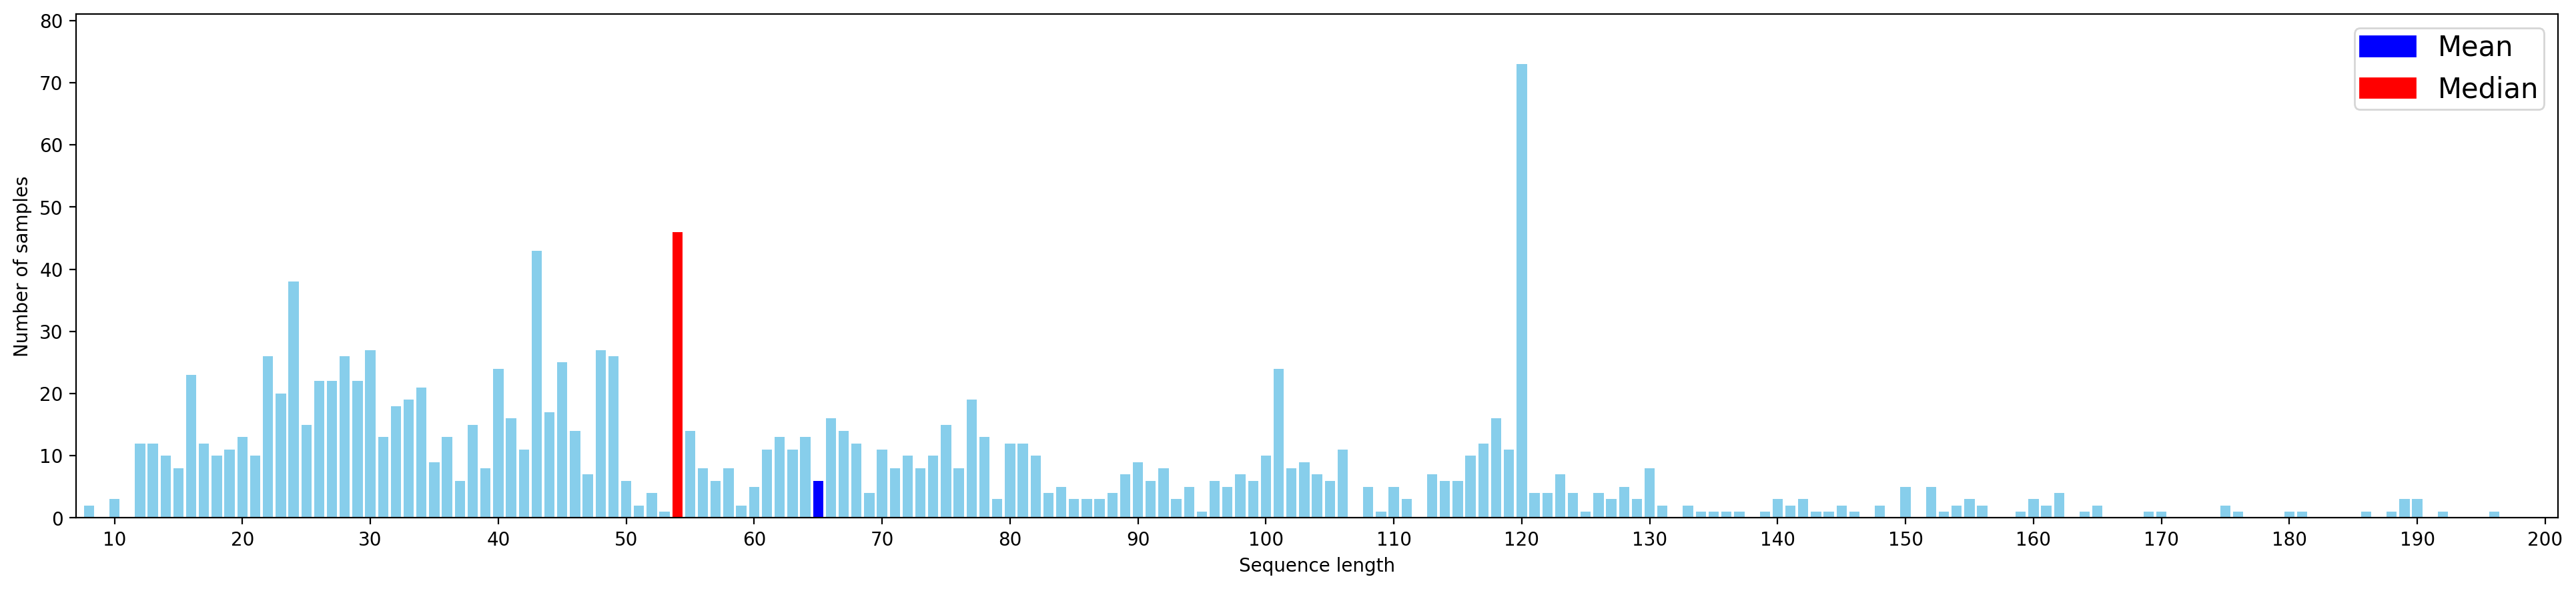
\includegraphics[width=\linewidth]{pics/plot_pks_distr.png}}
\caption{Analysis of Genegram-pks model compared with other tools }
\label{plots_pks}
\end{figure}

Similarly, we present the results of functional tests for this model and other tools in table~\ref{table_pks}. It can be seen that Watson-Crick pairs are predicted similarly to the main model, but wobble base pairs prediction accuracy decreased. However, the pseudoknotted structures processing was of particular interest in the context of Genegram-pks model and estimation by this criteria shows significant growth compared to the Genegram-main --- almost a quarter of all pseudoknots was detected perfectly, and about a half had small prediction errors. To sum up, this model generally losses to the main one, however, it shows very promising results in the aspect of pseudoknots detection being one of the best models for this problem.

\begin{table}
\centering
\caption{Genegram-pks and other models quality criteria measured on valid set}
\ra{1.4}
\begin{tabular}{@{}lccccccc@{}}\toprule
& \multicolumn{2}{c}{Pseudoknots} & \phantom{abc}& \multicolumn{3}{c}{Base pairs} \\
& No errors & 25\% errors  && Watson-Crick & GU & Others \\ \cmidrule{2-3} \cmidrule{5-7} 
Genegram-main  & 9 & 18 && 1628 & 61 & 47 \\
SPOT-RNA & 4 & 10 && 1893 & 173 & 71 \\
Ipknot & 2 & 5 && 1497 & 120 & 0 \\
Knotty & 11 & 20 && 1833 & 156 & 0 \\
RNAstructure & 3 & 7 && 1550 & 140 & 0 \\
PknotsRG & 11 & 20 && 1742 & 150 & 0 \\
HotKnots & 6 & 6 && 1621 & 143 & 0 \\
\bottomrule
Expected & 43 & 43 && 2407 & 258 & 156 \\
\bottomrule
\end{tabular}
\label{table_pks}
\end{table}

\subsubsection{Genegram-mps}
(NOT READY!)

Intresting object that our approach allows to consider without its explicit definition is a multiplet that appears when base pair starts to form bonds with other bases or base pairs. Multiplets are known to be functionally important, although, they are classified as tertiary structure features, so, secondary structure prediction tools are not usually able to can handle them. 

PDB provides more structural information, because it contains detailed crystallography result. The data is straight from nature: more variability in data --- more possibilities but harder to learn.

Experimental model that has possibilities in predicting more features of secondary and even tertiary structures.

For now it's more a discussion about the possibilities of our approach than really presentable result.

Multiplets have different typology, hard to estimate

(https://www.ncbi.nlm.nih.gov/pmc/articles/PMC6467009/) 

\subsubsection{Global tests}
In the previous sections we estimated three Genegram models separately on their validation sets and in this section, we provide some global tests for all the tools.

Due to the similar composition of training and validation sets for each model, the high results on validation make no reference to the general model quality, therefore, we downloaded several comparative and laboratory RNA secondary structure databases and evaluated Genegram models along with other tools on such data. These databases do not contain only purely selected structures, moreover, huge comparative databases usually aggregate a lot of homologous sequences with repetitive structural patterns, however, this experiment should check all models behavior on row data from various sources as opposed to the careful estimation on clean structures presented in the previous sections. We selected the following databases: CRW~\cite{cannone2002comparative}, Sprinzl~\cite{sprinzl1998compilation}, SRP~\cite{zwieb1992signal}, Rfam~\cite{griffiths2003rfam}, PDB~\cite{berman2000protein} (only single-chain samples without unmodelled bases) and Pseudobase~\cite{van2000pseudobase}. Note that most of these samples are completely new, however, some sequences or even databases could be previously used for some models training (e.g. Pseudobase was included in Genegram-pks training set). Table~\ref{table_all} represents the estimation of three Genegram models along with other tools by mean $F1$ score on all databases and the last column shows the mean $F1$ value among total samples. It can be seen that in most cases our models show adequate numbers regarding other tools, so, we can state that all neural networks generalize well on new datasets.

\begin{table}
\centering
\caption{All models estimation by $F1$ metrics on different databases}
\ra{1.4}
\begin{tabular}{@{}lcccccccc@{}}\toprule
& CRW & Sprinzl & SRP & Rfam & PDB & Pseudobase  & All data \\ \cmidrule{2-8} 
Genegram-main  & 69 & 73 & 59 & 43 & 74 & 42 & 69 \\
Genegram-pks  & 66 & 72 & 56 & 48 & 74 & 81 & 68 \\
Genegram-mps  &  &  &  &  &  &  &  \\
SPOT-RNA & 89 & 88 & 65 & 72 & 81 & 70 & 87 \\
Ipknot & 74 & 79 & 49 & 64 & 76 & 59 & 75 \\
Knotty & 74 & 75 & 63 & 63 & 79 & 76 & 74 \\
RNAstructure & 66 & 69 & 56 & 64 & 77 & 62 & 67 \\
PknotsRG & 62 & 61 & 65 & 66 & 79 & 77 & 62 \\
HotKnots & 61 & 60 & 66 & 66 & 78 & 61 & 61 \\
\bottomrule
Total samples & 11606 & 8777 & 360 & 1043 & 290 & 357 & 22433 \\
\bottomrule
\end{tabular}
\label{table_all}
\end{table}

Finally, we measured the time required for each tool to process fasta file with 100 RNA sequences and return secondary structure prediction for each sequence in its default output format. These tests were carried out on the workstation with the following characteristics: Ubuntu 20.04.2 LTS, Intel Core i5-10210U CPU 1.60GHz, NVIDIA GeForce MX250 GPU, and 7.5 GB RAM. We prepared two datasets by randomly selecting sequences from RNA STRAND database: the first set contained 100 sequences having lengths up to 100 and the second one --- 100 sequences with lengths up to 200. Table~\ref{table_time} shows the results of a performance experiment for such two fasta files. Genegram and SPOT-RNA were launched on GPU and the other tools have only CPU versions. It can be seen that the elapsed time spread among tools is quite big, moreover, several tools significantly lose in performance while processing longer sequences since various secondary structure prediction techniques may have completely different algorithmic complexity. However, Genegram shows an adequate performance due to the effective use of GPGPU in the parsing algorithm as well as in the neural network.

\begin{table}
\centering
\caption{Tools time performance on 100 sequences}
\ra{1.4}
\begin{tabular}{@{}lccc@{}}\toprule
& \multicolumn{2}{c}{\phantom{abc}  \phantom{abc}  \phantom{abc} Elapsed time, seconds}  \\
& Lengths 1-100 && Lengths 1-200  \\ \cmidrule{2-2} \cmidrule{4-4} 
Genegram & 28 && 39 \\
SPOT-RNA & 68 && 235 \\
Ipknot & 1 && 1 \\
Knotty & 283 && 3050 \\
RNAstructure & 10 && 15 \\
PknotsRG & 15 && 95 \\
HotKnots & 37 && 366 \\
\bottomrule
\end{tabular}
\label{table_time}
\end{table}